%% ID: A1986PIQ1l
%% TITLE: Force on table legs
%% TYPE: question
%% QUESTIONTYPE:  numerical
%% CONCEPTS: forces, vectors1, newtoni
%% VIDEOS: 
%% LEVEL: 2
%% TOPIC: mechanics/statics
%% ORDER: 6

\begin{problem}[Phil_table_forces]
{\exposition{A table consists of a circular wooden board of mass $m = 3$ kg resting on top of three vertical legs, each of mass $M = 0.5$ kg. The legs are equidistant from the centre of the table and form an equilateral triangle. Use $g = 9.8$ m s$^{-2}$.}
\begin{enumerate}
	\item  \question[a]{Find the magnitude of the reaction force from one of the legs on the tabletop.}
	\item  \question[b]{Find the magnitude of the reaction force from the ground on one of the legs.}
	\end{enumerate}
}
{\textit{Created for the Rutherford School Physics Project by PS.}}
{\begin{enumerate}
	\item
	\begin{figure} [h]
		\centering
		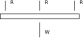
\includegraphics[width=0.4\textwidth]{Statics_table_top}
		\caption{}
		\label{fig:Statics_table_top}
	\end{figure}
	Figure \ref{fig:Statics_table_top} shows all of the forces acting on the tabletop. By symmetry, each of the legs exerts the same reaction force $R$. Resolving forces vertically gives us $3R = mg$, therefore $R = \frac{1}{3}mg = \frac{1}{3}\times 3 \times 9.8 = 9.8$ N.
	\answer{The magnitude of the reaction force from one of the legs on the tabletop is equal to \valuedef{R}{9.8}{N}.}
	\item
	\begin{figure} [h]
		\centering
		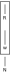
\includegraphics[width=0.05\textwidth]{Statics_table_leg}
		\caption{}
		\label{fig:Statics_table_leg}
	\end{figure}
	Figure \ref{fig:Statics_table_leg} shows all of the forces acting on one of the legs. Note that the reaction force from one of the legs on the tabletop is equal to the reaction force from the tabletop on one of the legs, and so they have both been marked as $R$; this is because the forces are a pair as described by Newton's third law, so must be equal in magnitude and opposite in direction. $N$ respresents the reaction force from the ground. Resolving vertically gives us $N = Mg + R = \left(0.5\times 9.8\right) + 9.8 = 14.7$ N.
	\answer{The magnitude of the reaction force from the ground on one of the legs is equal to \valuedef{N}{14.7}{N}.}
\end{enumerate}
}
\end{problem}